\esSezione{Riconoscitore della sequenza 101}\label{sec:esercizio3-1}

\begin{traccia}
Progettare, implementare in VHDL e testare mediante simulazione una macchina che riconosce la sequenza \texttt{101}. La macchina riceve un dato binario seriale $i$, un segnale di tempificazione $A$ e un segnale di modo $M$, e porta a '1' l'uscita $Y$ quando la sequenza viene riconosciuta. Se $M=0$ i bit sono valutati a gruppi di tre, senza sovrapposizione; se $M=1$ i bit sono valutati uno alla volta e la macchina torna allo stato iniziale a ogni riconoscimento (sequenze parzialmente sovrapposte).
\end{traccia}

\progetto

Il riconoscitore è una macchina a stati finiti di tipo Mealy, dal momento che l'uscita \texttt{y} dipende sia dallo stato corrente sia dall'ingresso \texttt{i}. È descritta con due process: uno combinatorio per la funzione di stato prossimo e di uscita, uno sincrono per il registro di stato. Il segnale di tempificazione \texttt{a} svolge il ruolo di clock della macchina e il reset \texttt{rst} è sincrono rispetto ad esso.

Gli stati sono sette, divisi in due sottografi, uno per modo, con lo stato iniziale \texttt{S0} in comune:
\begin{enumerate}
  \item modo 1 (un bit alla volta): \texttt{S0} (nessun bit utile), \texttt{S1} (visto '1'), \texttt{S2} (visto "10");
  \item modo 0 (gruppi di tre bit): \texttt{G1} (primo bit del gruppo pari a '1'), \texttt{G1E} (primo bit sbagliato), \texttt{G2} (letto "10"), \texttt{G2E} (gruppo ormai perso).
\end{enumerate}
In modo 0 gli stati terminano sempre dopo tre bit, con ritorno in \texttt{S0}, così da preparare il gruppo successivo. In modo 1, dopo il riconoscimento la macchina torna in \texttt{S0}; un '1' immediatamente successivo è quindi trattato come inizio di una nuova sequenza solo dal bit seguente, mentre l'autoanello su \texttt{S1} gestisce i '1' consecutivi. Il diagramma è riportato in figura~\ref{fig:esercizio3-1:stati}, con etichette nel formato \texttt{M i / Y}.

\begin{figure}[H]
  \centering
  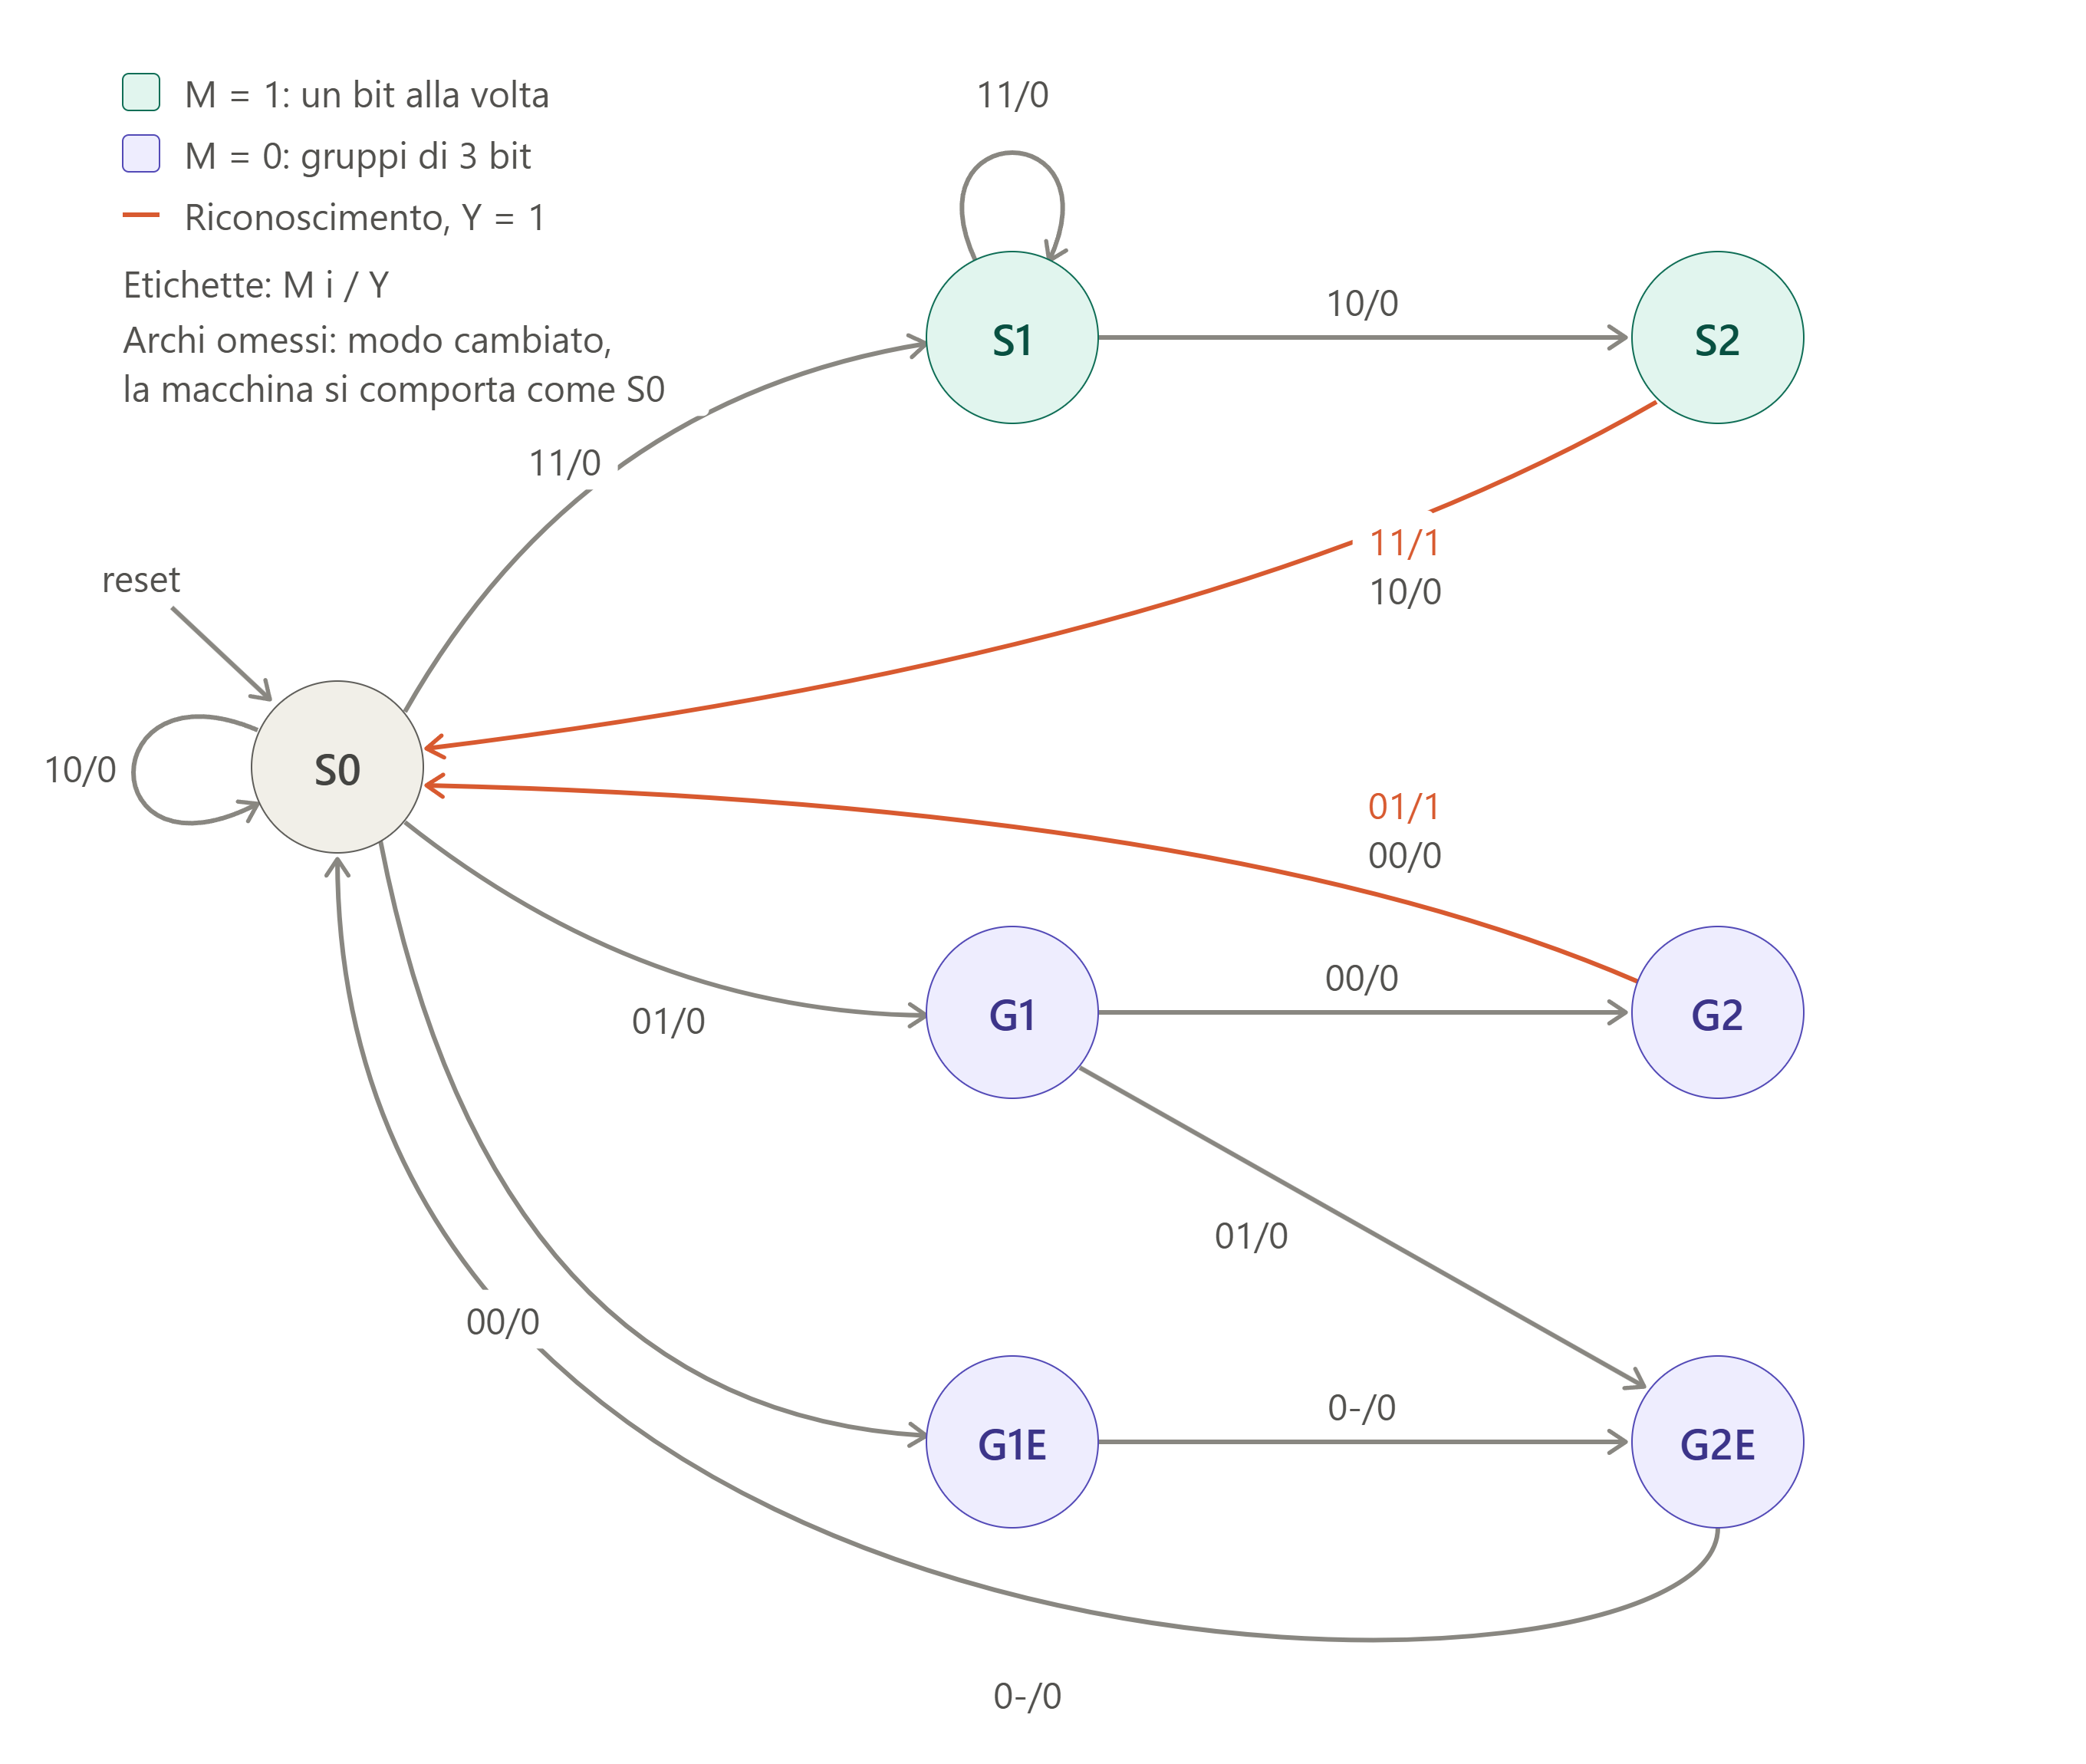
\includegraphics[width=0.75\linewidth]{figure/esercizio3-1/stati}
  \caption{FSM del riconoscitore 101}
  \label{fig:esercizio3-1:stati}
\end{figure}

Gli stati verdi appartengono al modo 1 e quelli viola al modo 0; l'arco arancione indica le transizioni con uscita a '1'. Gli archi nei quali il modo risulta cambiato rispetto allo stato in cui ci si trova sono omessi: in tal caso la macchina si comporta come se fosse in \texttt{S0} del nuovo modo, senza perdere il bit in ingresso.

\implementazione

L'entità \texttt{fsm\_sequence} ha cinque porte di tipo \texttt{std\_logic}: gli ingressi \texttt{i} (dato), \texttt{m} (modo), \texttt{a} (tempificazione) e \texttt{rst} (reset), e l'uscita \texttt{y}. L'architettura \texttt{Behavioral} definisce il tipo enumerato \texttt{state} con i sette stati e i segnali \texttt{current\_state} e \texttt{next\_state}.

Il process \texttt{f\_stato\_uscita} ha come sensitivity list \texttt{current\_state}, \texttt{m} e \texttt{i}. In testa assegna i valori di default: \texttt{y} a '0' e lo stato prossimo ottenuto come se la macchina fosse in \texttt{S0} per il modo corrente. Il costrutto \texttt{case} sullo stato corrente sovrascrive poi solo le transizioni diverse dal default, e ciascuna di esse è condizionata al modo coerente con lo stato: se \texttt{m} non lo è, resta valido il default e la macchina riparte come da \texttt{S0}. Il process \texttt{mem} è sensibile ad \texttt{a}: sul fronte di salita carica \texttt{S0} se \texttt{rst} vale '1', altrimenti \texttt{next\_state}.

\vhdlfile{esercizio3-1/fsm_sequence.vhd}{Implementazione del riconoscitore di sequenza}{lst:esercizio3-1:fsm}

\simulazione

Il testbench \texttt{fsm\_sequence\_tb} ha un'entità senza porte e istanzia il componente da verificare come \texttt{dut}. Il process \texttt{clk\_proc} genera il segnale \texttt{A} con periodo di \SI{10}{\nano\second} (costante \texttt{T}); il process \texttt{stim} applica gli ingressi, cambiando \texttt{i} a ogni periodo e riportando la macchina in reset tra un test e il successivo. Termina con un \texttt{wait} senza condizione. I test sono quattro:
\begin{enumerate}
  \item $M=1$, ingresso \texttt{010101}: la sequenza è riconosciuta al quarto bit; l'ultimo '1' non produce uscita;
  \item $M=0$, ingresso \texttt{010101}: il primo gruppo \texttt{010} non è valido, il secondo \texttt{101} è riconosciuto al sesto bit;
  \item $M=1$, ingresso \texttt{1101}: il riconoscimento avviene al quarto bit grazie all'autoanello su \texttt{S1};
  \item cambio di modo a metà sequenza: con $M=0$ si leggono \texttt{1} e \texttt{0}, poi $M$ passa a '1' e si leggono \texttt{1}, \texttt{0}, \texttt{1}; la macchina riparte da \texttt{S0} e riconosce la sequenza all'ultimo bit.
\end{enumerate}

\vhdlfile{esercizio3-1/fsm_sequence_tb.vhd}{Testbench del riconoscitore di sequenza}{lst:esercizio3-1:tb}

Il risultato della simulazione è mostrato in figura~\ref{fig:esercizio3-1:simulazione}.

\begin{figure}[H]
  \centering
  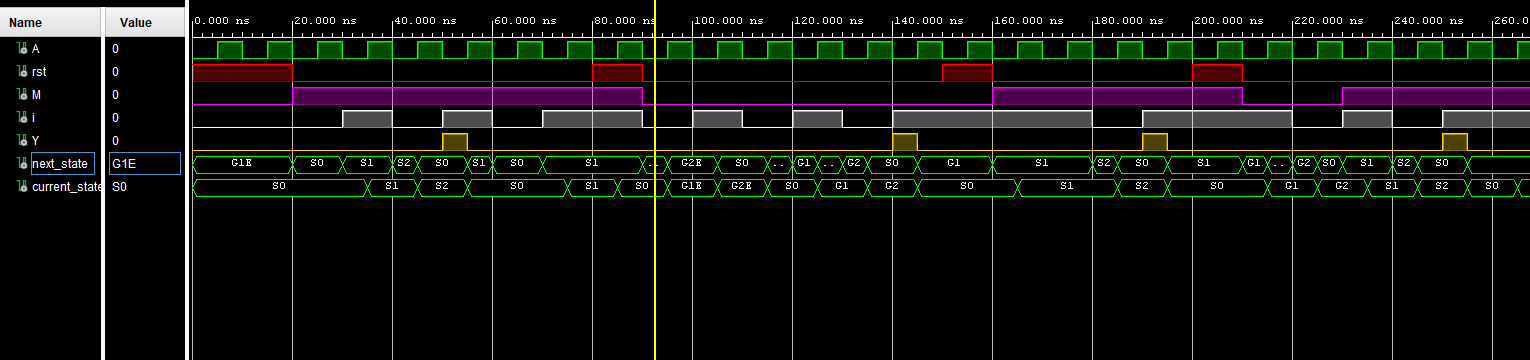
\includegraphics[width=\linewidth]{figure/esercizio3-1/simulazione}
  \caption{Simulazione del riconoscitore 101}
  \label{fig:esercizio3-1:simulazione}
\end{figure}

Consideriamo il primo test. Terminato il reset a \SI{20}{\nano\second}, con $M=1$ vengono applicati i bit \texttt{0}, \texttt{1}, \texttt{0}, \texttt{1}, uno per periodo di \texttt{A}: lo stato corrente passa da \texttt{S0} a \texttt{S1}, poi a \texttt{S2}. Quando il quarto bit, pari a '1', è presente in ingresso (intorno a \SI{50}{\nano\second}) la macchina è in \texttt{S2} e \texttt{Y} sale a '1'; al fronte di \texttt{A} successivo lo stato torna a \texttt{S0} e \texttt{Y} ridiventa '0'. Poiché \texttt{Y} dipende anche da \texttt{i}, l'uscita è un impulso della durata di mezzo periodo di \texttt{A}. Gli stessi impulsi si ritrovano nei tre test successivi, in corrispondenza dell'ultimo bit della sequenza riconosciuta.

\begin{risultato}
In tutti e quattro i test l'uscita \texttt{Y} assume il valore '1' una sola volta, in corrispondenza dell'ultimo bit della sequenza \texttt{101}.
\end{risultato}
